\documentclass{standalone}
\usepackage{tikz}
\usetikzlibrary{calc, intersections, decorations.pathreplacing}
\begin{document}
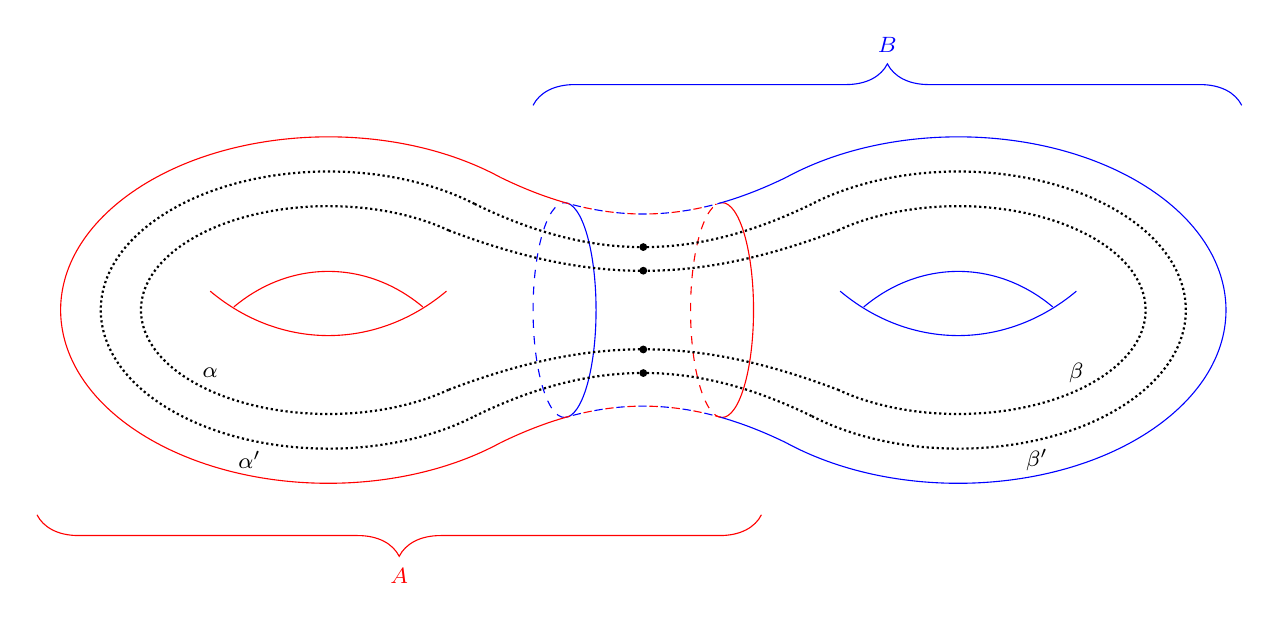
\begin{tikzpicture}[scale=2] % Syntax: [#1] optional arguments, (#2) center point, (#3:#4:#5) start angle, stop angle, radius; #6 secondary radius
  \def\centerarc[#1](#2)(#3:#4:#5)(#6){
    \draw[#1] ($(#2)+({#5*cos(#3)},{#6*sin(#3)})$) arc (#3:#4:#5 and #6);
  }

  \def\ltoruscolor{red}
  \def\rtoruscolor{blue}

  % Where to center the right torus
  \pgfmathsetmacro{\rtorusx}{4};
  \pgfmathsetmacro{\rtorusy}{0};

  % Parameters for drawing top half of left hole arc
  \pgfmathsetmacro{\lholetx}{.6};
  \pgfmathsetmacro{\lholety}{.02};

  % Bottom half of left hole arc
  \pgfmathsetmacro{\lholebx}{.75};
  \pgfmathsetmacro{\lholeby}{.12};

  % Parameters for drawing top half of right hole arc
  \pgfmathsetmacro{\rholetxl}{-\lholetx+\rtorusx};
  \pgfmathsetmacro{\rholetxr}{\lholetx+\rtorusx};
  \pgfmathsetmacro{\rholety}{\lholety+\rtorusy};

  % Bottom half of right hole arc
  \pgfmathsetmacro{\rholebxl}{-\lholebx+\rtorusx};
  \pgfmathsetmacro{\rholebxr}{\lholebx+\rtorusx};
  \pgfmathsetmacro{\rholeby}{\lholeby+\rtorusy};

  % Radius values for ellipse used to draw torus
  \pgfmathsetmacro{\rx}{1.7};
  \pgfmathsetmacro{\ry}{1.1};

  % Angles used for left torus --- left theta start, left theta finish
  \pgfmathsetmacro{\lts}{50};
  \pgfmathsetmacro{\ltf}{310};

  % Angles used for left torus --- left theta start, left theta finish
  \pgfmathsetmacro{\rts}{180+\lts};
  \pgfmathsetmacro{\rtf}{180+\ltf};

  % left X value for the connector
  \pgfmathsetmacro{\lconnx}{\rx * cos(\lts)};
  % left Y value for the connector
  \pgfmathsetmacro{\lconny}{\ry * sin(\lts)};

  % right X value for the connector
  \pgfmathsetmacro{\rconnx}{\rx * cos(\rts) + \rtorusx};
  % right Y value for the connector
  \pgfmathsetmacro{\rconny}{-\ry * sin(\rts) + \rtorusy};

  % Set the incoming / outgoing angles of elevation for the
  % connectors
  \pgfmathsetmacro{\connout}{26};
  \pgfmathsetmacro{\connin}{180-\connout};

  \pgfmathsetmacro{\bendamount}{40};

  % Left Hole
  \draw[\ltoruscolor] (-\lholetx, \lholety) to [bend left=\bendamount] (\lholetx, \lholety);
  \draw[\ltoruscolor] (-\lholebx, \lholeby)  to [bend right=\bendamount] (\lholebx, \lholeby);

  % Right Hole
  \draw[\rtoruscolor] (\rholetxl, \rholety) to [bend left=\bendamount] (\rholetxr, \rholety);
  \draw[\rtoruscolor] (\rholebxl, \rholeby)  to [bend right=\bendamount] (\rholebxr, \rholeby);

  \centerarc[\ltoruscolor](0,0)(\lts:\ltf:\rx)(\ry);
  \centerarc[\rtoruscolor](\rtorusx, \rtorusy)(\rts:\rtf:\rx)(\ry);

  % Define parameters for cut circles
  \pgfmathsetmacro{\cutoffset}{.5};
  \pgfmathsetmacro{\cutheight}{.682};

  % Solid right-hand cut
  \newcommand{\rcuts}{($(2,0)+(\cutoffset, -\cutheight)$) arc (-90:90:.2 and \cutheight)}
  \newcommand{\rcutd}{($(2,0)+(\cutoffset, -\cutheight)$) arc (270:90:.2 and \cutheight)}

  \newcommand{\lcuts}{($(2,0)+(-\cutoffset,-\cutheight)$) arc (-90:90:.2 and \cutheight)}
  \newcommand{\lcutd}{($(2,0)+(-\cutoffset,-\cutheight)$) arc (270:90:.2 and \cutheight)}

  % Right cut
  % dash this one
  \path[name path=rcut] \rcutd;
  \path \rcuts;

  % Left cut
  % dash this one
  \path \lcutd;
  \path[name path=lcut] \lcuts;

  \draw[\rtoruscolor] \lcuts;
  \draw[\rtoruscolor, dashed] \lcutd;
  \draw[\ltoruscolor] \rcuts;
  \draw[\ltoruscolor, dashed] \rcutd;

  % Store path info for top/bottom connectors
  \newcommand{\tconn}{(\lconnx, \lconny) to[out=-\connout, in=-\connin] (\rconnx, \rconny)}
  \newcommand{\bconn}{(\lconnx, -\lconny) to[out=\connout, in=\connin] (\rconnx, -\rconny)}

  % Get paths for top and bottom
  \path[name path=ptconn] \tconn;
  \path[name path=btconn] \bconn;

  % Find points of intersection between connector from right torus and
  % slicing circle (rct = right connector top)
  \path[name intersections={of=lcut and ptconn, by=lctp}];
  \path[name intersections={of=lcut and btconn, by=lcbp}];
  \path[name intersections={of=rcut and ptconn, by=rctp}];
  \path[name intersections={of=rcut and btconn, by=rcbp}];

  % \node[circle, fill, inner sep=1pt] (a) at (rctp) {};
  \begin{scope}
    \clip (lctp) -- ($(lctp) + (0,1)$) -- (0,\ry) -- (0,-\ry) -- ($(lcbp) - (0,1)$) -- cycle;
    \draw[\ltoruscolor] \tconn \bconn;
  \end{scope}

  \begin{scope}
    \clip (rctp) -- ($(rctp) + (0,1)$) -- (\rtorusx,\ry) -- (\rtorusx,-\ry) -- ($(rcbp) - (0,1)$) -- cycle;
    \draw[\rtoruscolor] \tconn \bconn;
  \end{scope}

  \begin{scope}
    \clip (rctp) -- (lctp) -- (lcbp) -- (rcbp) -- cycle;
    \draw[red,dash pattern=on 3pt off 5pt] \tconn \bconn;
    \draw[blue,dash pattern=on 3pt off 5pt, dash phase=4pt] \tconn \bconn;
  \end{scope}

  % Coordinate grid to make adjustments easier to eyeball
  % \draw[help lines, color=gray!30, dashed] (-1.9,-1.9) grid (6,2);
  % \draw[->] (-2,0)--(6,0) node[right]{$x$};
  % \draw[->] (0,-2)--(0,2) node[above]{$y$};

  \node[fill, circle, inner sep=1pt] (t1) at (2,.4) {};
  \node[fill, circle, inner sep=1pt] (a2) at (2,.25) {};
  \node[fill, circle, inner sep=1pt] (b2) at (2,-.25) {};
  \node[fill, circle, inner sep=1pt] (b1) at (2,-.4) {};

  \pgfmathsetmacro{\ascaledrx}{.85*\rx};
  \pgfmathsetmacro{\ascaledry}{.8*\ry};
  \pgfmathsetmacro{\ascaledlconnx}{\ascaledrx * cos(\lts)};
  \pgfmathsetmacro{\ascaledlconny}{\ascaledry * sin(\lts)};
  \pgfmathsetmacro{\ascaledrconnx}{\ascaledrx * cos(\rts) + \rtorusx};
  \pgfmathsetmacro{\ascaledrconny}{-\ascaledry * sin(\rts) + \rtorusy};
  \pgfmathsetmacro{\ascaledout}{26};
  \pgfmathsetmacro{\ascaledin}{180-\ascaledout};
  \newcommand{\ascaledtconn}{(\ascaledlconnx, \ascaledlconny) to[out=-\ascaledout, in=-\ascaledin] (\ascaledrconnx, \ascaledrconny)}
  \newcommand{\ascaledbconn}{(\ascaledlconnx, -\ascaledlconny) to[out=\ascaledout, in=\ascaledin] (\ascaledrconnx, -\ascaledrconny)}

  \draw[thick, densely dotted] \ascaledtconn \ascaledbconn;
  \centerarc[thick, densely dotted](0,0)(\lts:\ltf:\ascaledrx)(\ascaledry);
  \centerarc[thick, densely dotted](\rtorusx,\rtorusy)(\rts:\rtf:\ascaledrx)(\ascaledry);

  \pgfmathsetmacro{\bscaledrx}{.7*\rx};
  \pgfmathsetmacro{\bscaledry}{.6*\ry};
  \pgfmathsetmacro{\bscaledlconnx}{\bscaledrx * cos(\lts)};
  \pgfmathsetmacro{\bscaledlconny}{\bscaledry * sin(\lts)};
  \pgfmathsetmacro{\bscaledrconnx}{\bscaledrx * cos(\rts) + \rtorusx};
  \pgfmathsetmacro{\bscaledrconny}{-\bscaledry * sin(\rts) + \rtorusy};
  \pgfmathsetmacro{\bscaledout}{20.8};
  \pgfmathsetmacro{\bscaledin}{180-\bscaledout};
  \newcommand{\bscaledtconn}{(\bscaledlconnx, \bscaledlconny) to[out=-\bscaledout, in=-\bscaledin] (\bscaledrconnx, \bscaledrconny)}
  \newcommand{\bscaledbconn}{(\bscaledlconnx, -\bscaledlconny) to[out=\bscaledout, in=\bscaledin] (\bscaledrconnx, -\bscaledrconny)}

  \draw[thick, densely dotted] \bscaledtconn \bscaledbconn;
  \centerarc[thick, densely dotted](0,0)(\lts:\ltf:\bscaledrx)(\bscaledry);
  \centerarc[thick, densely dotted](\rtorusx,\rtorusy)(\rts:\rtf:\bscaledrx)(\bscaledry);

  \node (alpha1) at (-.75, -.4) {\footnotesize $\alpha$};
  \node (alpha2) at (-.5, -.95) {\footnotesize $\alpha'$};

  \node (beta1) at (4.75, -.4) {\footnotesize $\beta$};
  \node (beta2) at (4.5, -.95) {\footnotesize $\beta'$};

  \draw[
    red,
    decorate,
    decoration={
      brace,
      amplitude=15pt
    },
    % xshift=-4pt,
    % yshift=-10pt
  ] (2.75,-1.3) -- (-1.85,-1.3)  node [midway, yshift=-22pt] {\footnotesize $\color{red} A$};

  \draw[
    blue,
    decorate,
    decoration={
      brace,
      amplitude=15pt
    },
    % xshift=-4pt,
    % yshift=-10pt
  ] (1.3,1.3) -- (5.8,1.3)  node [midway, yshift=22pt] {\footnotesize $\color{blue} B$};

  % \draw[densely dashed, very thin] (t1) -- (.7,)

  % \draw[densely dotted] (2,.3) .. controls (1.3,.5) .. (1.15,.2) .. controls (1.1,-.1) .. (1.5,-.1) .. controls (2.2,-.4) .. (2,.3);

\end{tikzpicture}
\end{document}